\ffigbox[\FBwidth]{%
\caption{\centering La famille d'Oedipe}\label{Fig:oedipe_tree}
}{
    \fbox{
        \begin{tikzpicture}[every node/.style={font=\small}]

            % =========================
            % STYLES
            % =========================
            \tikzset{
                H/.style={text=blue},
                F/.style={text=orange!90!black},
                person/.style={align=center},
            }

            % =========================
            % NODES (COORDINATES)
            % =========================

            % Top generation - crown scaled much smaller to match \faCrown size
            \node[person,H] (Agenor) at (0,0) {Agenor \raisebox{3pt}{\scalebox{0.35}{\pgfornament{147}}}};

            % Cadmos + Harmonie
            \node[person,H] (Cadmos)   at (-2,-1.5) {Cadmos \faCrown};
            \node[person,F]        (Harmonie) at ( 2,-1.5) {Harmonie};

            % Children of Cadmos - increased spacing
            \node[person,F] (Ino)    at (-4.5,-3) {Ino};
            \node[person,F] (Agave)  at (-2,-3) {Agavé};
            \node[person,H] (Polydore) at (0,-3) {Polydore};
            \node[person,F] (Nictis) at (2,-3) {Nictéis};

            % Agave line
            \node[person,H] (Penthe)  at (-2,-4.2) {Penthée \faCrown};
            \node[person,H] (Oclosos) at (-2,-5.4) {Oclosos};
            \node[person,H] (Menecee) at (-2,-6.6) {Ménecée};

            % Children of Ménecée: Creon & Jocaste
            \node[person,H] (Creon) at (-4,-7.8) {Créon \faCrown};
            \node[person,F]           (Jocaste) at (0,-7.8) {Jocaste};

            \node[person,F] (Eurydice) at (-6,-7.8) {Eurydice};
            \node[person,H] (Hemon)    at (-4,-9.3) {Hémon};

            % Jocaste + Oedipe
            \node[person,H] (Oedipe) at (2,-7.8) {Œdipe \faCrown};

            % Children of Jocaste & Oedipe (shared) - increased spacing
            \node[person,F] (Antigone) at (0,-9.3) {Antigone};
            \node[person,F] (Ismene)   at (1.8,-9.3) {Ismène};
            \node[person,H] (Eteocle)  at (3.6,-9.3) {Étéocle \faCrown};
            \node[person,H] (Polynice) at (5.4,-9.3) {Polynice};

            % Increased spacing between Ladamos and Thersandre
            \node[person,H] (Ladamos)   at (3.6,-10.8) {Ladamos \faCrown};
            \node[person,H] (Thersandre) at (5.4,-10.8) {Thersandre};

            % Polydore line
            \node[person,H] (Labdacos) at (0,-4.2) {Labdacos};
            \node[person,H] (Laios)    at (0,-5.4) {Laïos};

            % =========================
            % CONNECTIONS (using anchor points and aligned junctions)
            % =========================

            % Agenor → Cadmos
            \draw (Agenor.south) -- (Cadmos.north);

            % Cadmos + Harmonie → children (all at same y-level)
            \coordinate (CadmosHarmonieJunction) at (0,-2.25);
            \draw (Cadmos.south) -- (Cadmos.south |- CadmosHarmonieJunction) -- (CadmosHarmonieJunction);
            \draw (Harmonie.south) -- (Harmonie.south |- CadmosHarmonieJunction) -- (CadmosHarmonieJunction);
            \draw (CadmosHarmonieJunction) -| (Ino.north);
            \draw (CadmosHarmonieJunction) -| (Agave.north);
            \draw (CadmosHarmonieJunction) -| (Polydore.north);

            % Agave line
            \draw (Agave.south) -- (Penthe.north);
            \draw (Penthe.south) -- (Oclosos.north);
            \draw (Oclosos.south) -- (Menecee.north);

            % Ménecée → Creon & Jocaste (aligned junction)
            \coordinate (MeneceeJunction) at (-2,-7.2);
            \draw (Menecee.south) -- (MeneceeJunction);
            \draw (MeneceeJunction) -| (Creon.north);
            \draw (MeneceeJunction) -| (Jocaste.north);

            % Creon + Eurydice → Hemon (aligned junction)
            \coordinate (CreonEurydiceJunction) at (-5,-8.6);
            \draw (Eurydice.south) -- (Eurydice.south |- CreonEurydiceJunction) -- (CreonEurydiceJunction);
            \draw (Creon.south) -- (Creon.south |- CreonEurydiceJunction) -- (CreonEurydiceJunction);
            \draw (CreonEurydiceJunction) -- (Hemon.north);

            % Polydore + Nictis → Labdacos (aligned junction)
            \coordinate (PolydoreNictisJunction) at (1,-3.6);
            \draw (Polydore.south) -- (Polydore.south |- PolydoreNictisJunction) -- (PolydoreNictisJunction);
            \draw (Nictis.south) -- (Nictis.south |- PolydoreNictisJunction) -- (PolydoreNictisJunction);
            \draw (PolydoreNictisJunction) -- (Labdacos.north);
            
            \draw (Labdacos.south) -- (Laios.north);

            % Laios → Oedipe
            \draw (Laios.south) -- ++(0,-0.5) -| (Oedipe.north);

            % Jocaste ↔ Oedipe (couple - horizontal line)
            \draw (Jocaste.east) -- (Oedipe.west);

            % Their children (converge at common point at same y-level)
            \coordinate (JocasteOedipeJunction) at (1,-8.6);
            \draw (Jocaste.south) -- (Jocaste.south |- JocasteOedipeJunction) -- (JocasteOedipeJunction);
            \draw (Oedipe.south) -- (Oedipe.south |- JocasteOedipeJunction) -- (JocasteOedipeJunction);
            
            \draw (JocasteOedipeJunction) -| (Antigone.north);
            \draw (JocasteOedipeJunction) -| (Ismene.north);
            \draw (JocasteOedipeJunction) -| (Eteocle.north);
            \draw (JocasteOedipeJunction) -| (Polynice.north);

            % Children of Eteocle / Polynice
            \draw (Eteocle.south) -- (Ladamos.north);
            \draw (Polynice.south) -- (Thersandre.north);

            % =========================
            % LEGEND
            % =========================
            \node[draw, thick, fill=white, align=left, font=\footnotesize, 
            inner sep=8pt, anchor=north west] at (-7,0.5) {
                \textbf{Légende :} \\[3pt]
                \textcolor{blue}{Bleu} = Homme \\[2pt]
                \textcolor{orange!90!black}{Orange} = Femme \\[2pt]
                \faCrown\ = Roi de Thèbes \\[2pt]
                \raisebox{3pt}{\scalebox{0.35}{\pgfornament{147}}} = Roi de Tyr
            };

        \end{tikzpicture}
    }
}